\section{Data}
\label{sec:data}

We train on the pretraining corpus of GIFT-Eval~\citep{aksu2024gifteval}
and we evaluate on the GIFT-Eval benchmark. The authors of GIFT-Eval
built this corpus with no overlap with the test split of the
benchmark. Each batch also holds a few synthetic series, and a mixup
step mixes the series of some batches.

\paragraph{Benchmark.}
GIFT-Eval has $23$ datasets with frequencies from $10$ seconds to one
year. They cover, for example, electricity load, solar power, weather,
road traffic, cloud servers, air quality, river flow, hospital
admissions, sales and the economic series of M4. Each dataset has up to
three forecast terms. The short term has a horizon set by the
frequency, for example $48$ steps for hourly data. The medium and long
terms have $10$ and $15$ times this horizon, and only $21$ pairs of a dataset
and a frequency, all hourly or finer, have them. A configuration is one dataset at one
frequency and one term, and the benchmark has $97$ configurations.

\paragraph{Real series.}
The pretraining corpus, GiftEvalPretrain, has $152$ sources,
$3.3$ million rows and $231$ billion values. We sample it with the
method of Moirai~\citep{woo2024moirai}. A source is drawn with a
probability proportional to its number of rows times the weight of the
source in the Moirai training mix. A row is drawn with a probability
proportional to its length (the ERA5 and CMIP6 sources draw their rows
uniformly, as in Moirai), and a window of $1024$ values starts at a
uniform position in the row. A draw keeps a random subset of the
variates of the row, as in Moirai, and each kept variate becomes a
separate univariate series. The covariates of a row train like its
target variates. A series shorter than the window gets zeros on its
left, and the normalisation of Section~\ref{sec:normalisation} treats
these zeros as padding. A run of $166{,}000$ steps reads $251$ real
windows at each step: $42$ million windows, or $43$ billion window
values. This is $18.5\%$ of the values of the corpus. The zero padding
is about a tenth of the window values, so the run reads about $38$
billion real values.

\paragraph{Synthetic series.}
Each batch holds two synthetic series, a \emph{forked ARMA} pair. The
two series share one past and have two different futures. We draw the
orders $p, q$ uniformly in $\{1, \ldots, 8\}$ and the coefficients
from a standard normal distribution, then we rescale each coefficient
set to an $\ell_1$ norm of at most $0.95$. This bound is a
sufficient condition for a stationary AR part and an invertible MA
part. The two series follow the same ARMA path
with unit Gaussian noise up to a fork point, drawn uniformly between
one quarter and three quarters of the window. After the fork, each
series continues from the shared state with its own noise, and with
its own copy of the coefficients plus a Gaussian perturbation of
standard deviation $0.05$. The perturbed coefficients are clipped to
the same $\ell_1$ bound, and the shared path starts after a burn-in of
$200$ steps. Each series is the cumulative sum of its
ARMA path, so it is an ARIMA$(p, 1, q)$ series.
Figure~\ref{fig:forked-arma} shows one pair.

\begin{figure}[t]
  \centering
  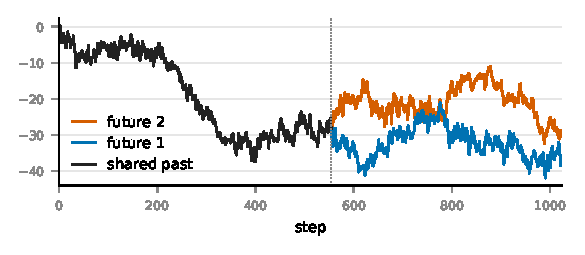
\includegraphics[width=0.6\linewidth]{figures/synthetic_forked_arma.pdf}
  \caption{A forked ARMA pair: one shared past, then two futures after
    the fork (dotted line).}
  \label{fig:forked-arma}
\end{figure}

\paragraph{Crossfade series.}
Each batch also holds three series built from two real windows $A$ and
$B$ of the batch: $A$ and $B$, each normalised to zero mean and unit
variance, and their crossfade
\[
  C_t \;=\; (1 - s_t)\, A_t \;+\; s_t\, B_t .
\]
The weight $s_t$ goes linearly from $0$ to $1$ over a transition
around a midpoint. The midpoint is uniform in the window, and the
width of the transition is log-uniform between $1/128$ of the window
and the full window (Figure~\ref{fig:crossfade}).

The batch is the same at every step: $256$ series, of which $251$ real
windows, the forked ARMA pair and the three crossfade series
($251 + 2 + 3 = 256$).

\begin{figure}[t]
  \centering
  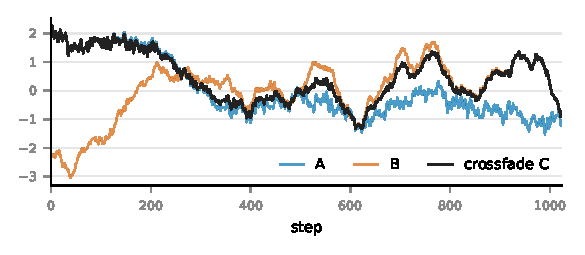
\includegraphics[width=0.6\linewidth]{figures/synthetic_crossfade.pdf}
  \caption{A crossfade $C$ of two series $A$ and $B$. In training, $A$
    and $B$ are real windows of the batch. Here $A$ is the first future
    of Figure~\ref{fig:forked-arma} and $B$ is one more ARIMA draw, and
    the transition is wide so that the blend is visible.}
  \label{fig:crossfade}
\end{figure}

\paragraph{Mixup.}
At each step, with probability $0.3$, we mix the whole batch with the
mixup of~\citet{zhang2018mixup}. We draw one weight
$a \sim \mathrm{Beta}(0.2, 0.2)$ and one random permutation $\pi$ of
the batch, and each series $x_b$ becomes
\[
  \tilde{x}_b \;=\; a\, x_b \;+\; (1 - a)\, x_{\pi(b)} .
\]
The frequency and seasonality embeddings of
Section~\ref{sec:scale-embedding} mix with the same weight. The mixup
acts on the raw values, before the normalisation. A mixed series keeps
the longer zero padding of its two series. The TSMixup of
Chronos~\citep{ansari2024chronos} mixes up to $k$ series after a
scaling of each series; our mixup mixes two raw series. Before the
mixup, each series changes sign with probability $0.5$.


